\documentclass[14pt, a4paper]{extarticle}
%\usepackage{graphicx}
\usepackage{array}
\usepackage{ulem}
\usepackage[T2A]{fontenc}
\usepackage[utf8]{inputenc}
\usepackage[english,russian]{babel}
\usepackage{color}

\usepackage[section]{placeins}

\usepackage{times}
\usepackage[top=2cm, bottom=2cm, left=3cm, right=1.5cm]{geometry}
% PDF Search & cut'n'paste
\usepackage{cmap}

% Indent the first paragraph as well
\usepackage{indentfirst}

% According to GOST, sections should be called chapters in diploma
\usepackage{titlesec}

% Detect whether PDFLaTeX is in use
\usepackage{ifpdf}

% Graphics
\ifpdf
    \usepackage[pdftex]{graphicx}
\else
    \usepackage{graphicx}
\fi

% Hyperlinks
\ifpdf
        \usepackage[pdftex]{hyperref}
\else
        \usepackage{hyperref}
\fi

\hypersetup{
        unicode=true,
        pdftitle={
        },
        pdfauthor={},
        pdfkeywords={
        },
        colorlinks,
        citecolor=black,
        filecolor=black,
        linkcolor=black,
        urlcolor=blue
}

% Russian-styled figure and table captions
\usepackage[labelsep=period]{caption}
% This declaration makes TeX less fussy about line breaking. This can
% prevent overfull boxes, but may leave too much space between words.
% As this really isn't a fine art typography, we'll turn it on, so
% we won't have paragraphs which spans on the margins...
\sloppy

% Page numbering at the right topmost part of the page
% \pagestyle{myheadings}

\usepackage{listings}
\let\stdsection\section
\renewcommand\section{\newpage\stdsection}
\definecolor{lightgray}{rgb}{.9,.9,.9}
\definecolor{darkgray}{rgb}{.4,.4,.4}
\definecolor{purple}{rgb}{0.65, 0.12, 0.82}
\graphicspath{{./images/}}
\lstdefinelanguage{JavaScript}{
  keywords={typeof, new, true, false, catch, function, return, null, catch, switch, var, if, in, while, do, else, case, break},
  keywordstyle=\color{blue}\bfseries,
  ndkeywords={class, export, boolean, throw, implements, import, this},
  ndkeywordstyle=\color{darkgray}\bfseries,
  identifierstyle=\color{black},
  sensitive=false,
  comment=[l]{//},
  morecomment=[s]{/*}{*/},
  commentstyle=\color{purple}\ttfamily,
  stringstyle=\color{red}\ttfamily,
  morestring=[b]',
  morestring=[b]"
}
\lstset{
   language=JavaScript,
   backgroundcolor=\color{lightgray},
   extendedchars=true,
   basicstyle=\footnotesize\ttfamily,
   showstringspaces=false,
   showspaces=false,
   numbers=left,
   numberstyle=\footnotesize,
   numbersep=9pt,
   tabsize=2,
   breaklines=true,
   showtabs=false,
   captionpos=b
}
\linespread{1.5}

%% TODO Нормальная титульная страница
\author{OverMMaTeX}
\title{Cosmology 101}
\date{\today}

%% ==========================================================
%          _____ _______  _______
%         |_   _| ____\ \/ /_   _|
%           | | |  _|  \  /  | |
%           | | | |___ /  \  | |
%           |_| |_____/_/\_\ |_|
%
%% ==========================================================
\begin{document}

%\maketitle
\thispagestyle{empty}
\begin{center}
OverMMaTeX\\
Mathematica + LaTeX [online]\\
\end{center}
%\vspace{1cm}
\begin{center}
Creación de documentos cientificos en linea\\
\end{center}
\vspace{2cm}
\begin{center}
    \Large{OverMMaTex - Cosmology 101} \\
\end{center}
\vspace{1cm}
\begin{center}
    \normalsize{Manual de uso} \\
    \large{Instrucciones}
\end{center}
\vspace{3cm}
\noindent
%\begin{center}
%    \small
%    \begin{tabular}{lcl}
%        Научный руководитель & \dotuline{\phantom{кошерная подпись}} & старший преподаватель\\
%        & /подпись/ & Антипов И.Г.\\
%        Рецензент & \dotuline{\phantom{кошерная подпись}} & аспирант \\
%        & /подпись/& Петров А.Г. \\
%        ``Допустить к защите'' & \dotuline{\phantom{кошерная подпись}} & д.ф.-м.н., проф. Терехов А.Н. \\
%        заведующий кафедрой, & /подпись/& \\
%    \end{tabular}
%\end{center}
%\vspace{\fill}
%\begin{center}
    \small
    From MMaTeX\\2025
\end{center}
\pagebreak

\include{title-en}

\setcounter{page}{1}
\tableofcontents
\newpage

\section{Introduction}

vamos a ver como funciona esto

Una figura

\begin{figure}[htb]
\centering
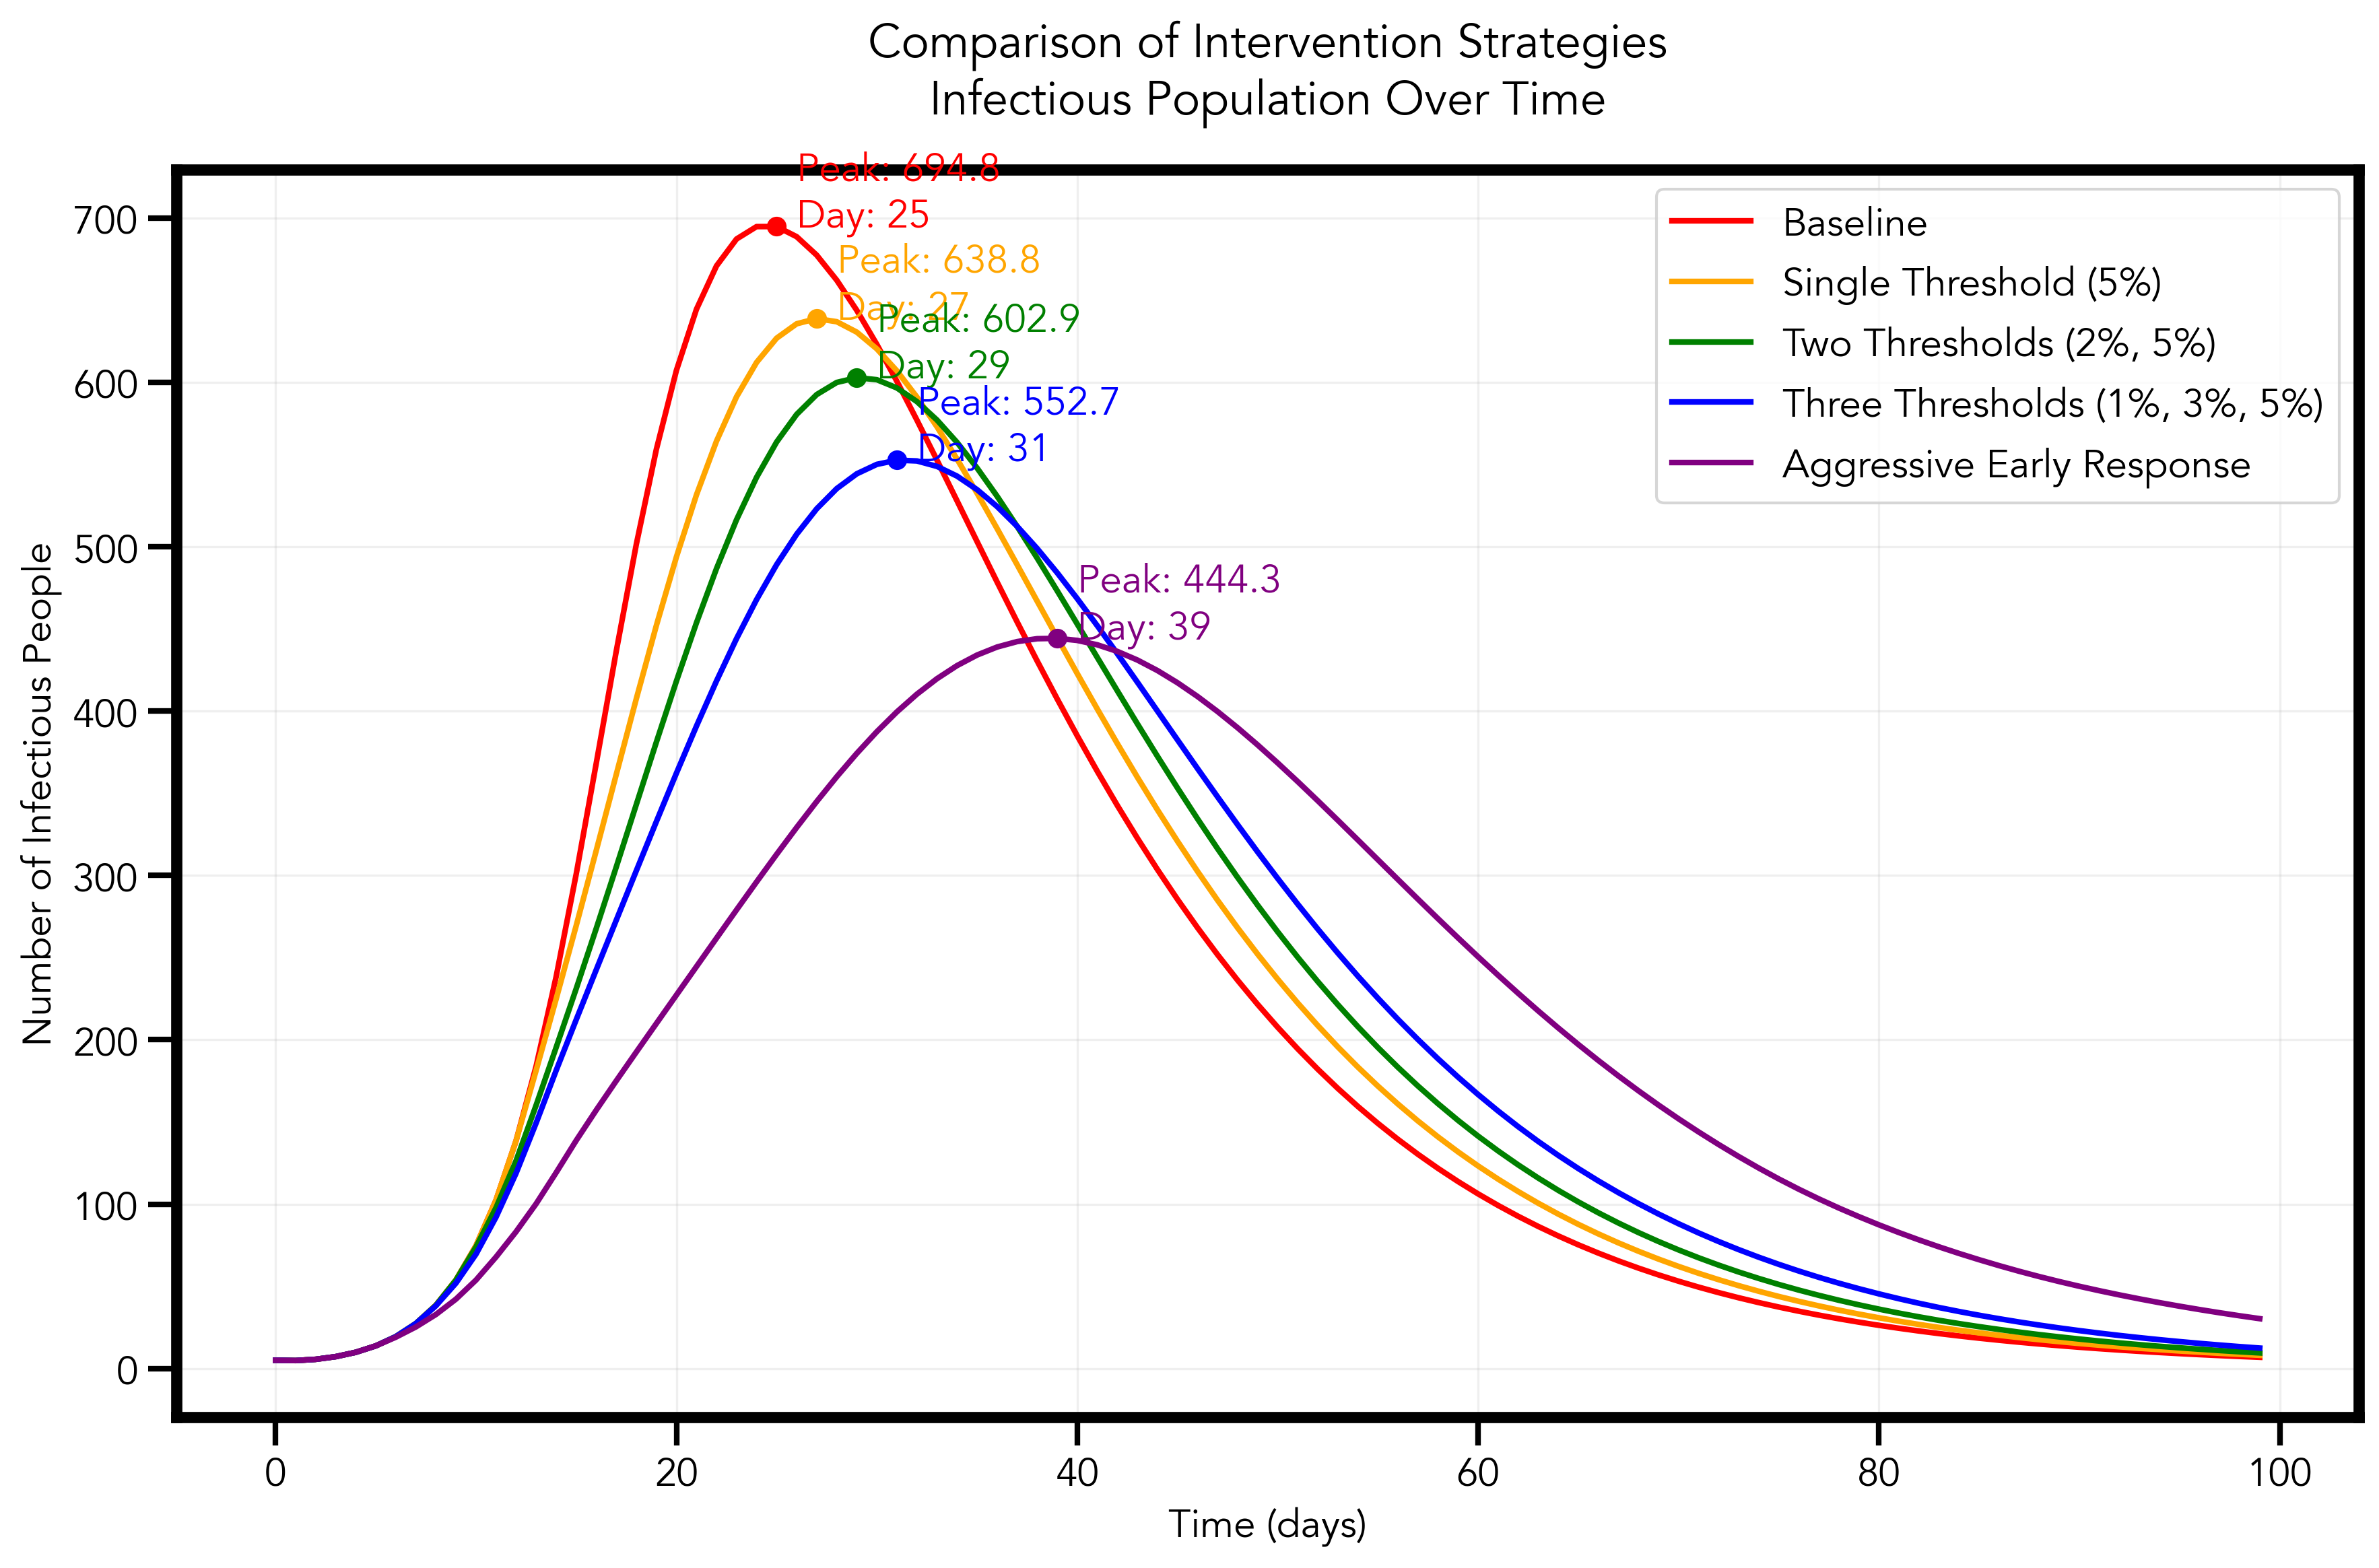
\includegraphics[width=1.0\textwidth]{./images/seir_comparison.png}
\caption{Mi figura 1}
\label{fig:seir1}
\end{figure}



%\include{architecture-1}

%\include{impl}

%\include{algo}

%\include{testing-algos}

%\include{architecture-2}

%\include{testing-rc}

%\include{mirror}

%\include{outro}

\begin{thebibliography}{9}

\bibitem{webgl}
  Спецификация WebGL \\
  \emph{http://www.khronos.org/webgl}.

\bibitem{nodejs}
  Официальный сайт Node.js \\
  \emph{http://nodejs.org/}

\bibitem{expressjs}
  Официальный сайт Express.js \\
  \emph{http://expressjs.com/}

\bibitem{threejs}
  Официальный репозиторий Three.js \\
  \emph{https://github.com/mrdoob/three.js/}

\bibitem{thrift}
  Официальный сайт Apache Thrift \\
  \emph{http://thrift.apache.org/}

\bibitem{nodethriftpatch}
  Ветка проекта node-thrift с исправленной ошибкой \\
  \emph{https://github.com/aslushnikov/node-thrift}

\bibitem{jade}
  Официальный сайт Jade \\
  \emph{http://jade-lang.com/}

\bibitem{jquery}
  Официальный сайт JQuery \\
  \emph{http://jquery.com/}

\bibitem{jqueryform}
  Описание проекта JQuery Form \\
  \emph{http://jquery.malsup.com/form/}

\bibitem{underscore}
  Официальный сайт Underscore \\
  \emph{http://documentcloud.github.com/underscore/}

\bibitem{webgl-shaders}
  Введение в WebGL. Шейдеры. \\
  \emph{http://learningwebgl.com/blog/?p=28}

\bibitem{observer}
  Шаблон проектирования Observer \\
  \emph{http://en.wikipedia.org/wiki/Observer\_pattern}

\bibitem{strategy}
  Шаблон проектирования Strategy \\
  \emph{http://en.wikipedia.org/wiki/Strategy\_pattern}

\bibitem{http10}
  Методы HTTP 1.0 \\
  \emph{http://www.w3.org/Protocols/HTTP/1.0/draft-ietf-http-spec.html\#Methods }

\end{thebibliography}

\end{document}

